\section{Cryptocurrencies \& the blockchain} \label{cryptocurrencies-the-blockchain}

One especially noteworthy contemporary application for cryptography is in the construction of blockchains, which form the basis of cryptocurrencies and smart contract platforms. Conventionally, electronic transactions relied on trusted authorities for authorisation. For example, in a regular online bank transaction the bank itself acts as the trusted authority. This requires absolute trust in a centralised agency.

The goal of blockchain technology is to enable transactions in a trustless environment where there is no centralised, trusted authority. This requires \emph{distributed consensus algorithms} to replace trusted authorities. For this to function in a self-regulating manner there must be mechanisms to both incentivise nodes to participate in consensus, but in a way that prevents collusion and ensures honesty.

\subsection{Proof of work (PoW)}

Proof of work is an approach for randomly choosing a subset of nodes in a network to participate in consensus. In the Bitcoin protocol \cite{bib:NakamotoS} this is referred to as \emph{coin mining}. Proof of work has two purposes:
\begin{itemize}
	\item Who it is that successfully mines coins and participates in subsequent consensus should be inherently randomised to prevent conspiratorial behaviour.
	\item The problem should inherently waste time, so-called `friction'. This restricts the number of nodes likely to succeed. Bitcoin chooses to do this by making users solve inverse hashing problems, whereby an input string to a hash function is deemed to be a coin if its hash has a certain number of leading zeros. As discussed previously, inverse hashing is inherently prohibitive owing to the pre-image resistance of hash functions. Rather than requiring inverting a complete hash we instead require finding a hash output with some adjustable number of leading zeroes, which tune the likelihood of finding a satisfying pre-image, a so-called \emph{partial pre-image} problem. This is how monetary policy is effectively enforced in such protocols where this \emph{difficulty parameter} controls monetary expansion. Specifically, for,
		\begin{align} \label{eq:pow_1}
			x=\mathrm{hash}(y),
		\end{align}
		we wish to find a $y$ such that,
		\begin{align} \label{eq:pow_2}
			x_{1\dots d}=\{0,\dots,0\},
		\end{align}
		where $d$ is the difficulty parameter.
\end{itemize}

In the Bitcoin protocol $x$ is derived from a hash of the  transaction history, such that PoW mining is always unique and associated with the verification of a given transaction.

Due to the unstructured nature of the partial pre-image problem, classical techniques for PoW mining simply rely on brute-force, repeatedly hashing random bit-strings until a satisfying one is found. For difficulty parameter $d$, the likelihood of a single randomly chosen $y$ satisfying Eqs.~\eqref{eq:pow_1} \& \eqref{eq:pow_2} is,
\begin{align}
	P=2^{-d},
\end{align}
and the average number of hashing operations required until a satisfying one is found is,
\begin{align}
	N = \frac{1}{P} = 2^d.	
\end{align}
This enforces our requirement that the choice of nodes participating in the consensus be a small, random subset of nodes and therefore unlikely to be able to collude.

Grover's algorithm (Sec.~\ref{grovers-algorithm}) provides some, albeit limited, quantum advantage here. Although quantum computers cannot efficiently perform inverse hashing, Grover's algorithm has the ability to provide a polynomial speedup in this process by treating inverse hashing as a satisfiability problem. Grover's algorithm in the absence of fault-tolerance overheads provides a quadratic speedup here. What does this translate to in terms of mining? If ordinarily a classical computer would require $2^d$ attempts to successfully find a new coin, a quantum computer could do so using, 
\begin{align}
	O(\sqrt{2^d})=O(2^{d/2}),
\end{align}
	attempts. Although this translates to faster mining, this can be offset by adjusting the difficulty parameter $d$, specifically by doubling it.

Note that proof-of-work is not the only consensus algorithm utilised in blockchains. Indeed, a major criticism of proof-of-work is that the associated friction necessarily wastes compute cycles, resulting in high energy consumption\footnote{The energy consumption associated with the mining necessary to maintain the Bitcoin network is estimated to be on the order of that consumed by a small country, while a single Bitcoin transaction is estimated to consume around \href{https://www.cnet.com/personal-finance/crypto/bitcoin-mining-how-much-electricity-it-takes-and-why-people-are-worried/}{1,449kWh of energy} at the time of writing.}. For this reason many contemporary blockchains have switched to alternate consensus mechanisms such as \emph{proof-of-stake}, whereby participants wager currency to participate in consensus. However proof-of-stake, despite being far more time and energy efficient\footnote{Ethereum's transition to proof-of-stake is touted as being around 99\% more energy efficient than its previous proof-of-work approach.}, is less secure than proof-of-work as it does not ensure randomisation of consensus participants to the extent that proof-of-work does, thereby making it more vulnerable to collusion\footnote{Consensus via a majority vote can be falsified if the majority of participants collude, the so-called `51\% attack'.}.

(??? results from Brennen/Tomamichel on time required to break
blockchains)

\subsection{Distributed consensus}

The proof of work concept is utilised in distributed consensus to randomise which nodes participate. When combined with a reward system, nodes are incentivised to join this lottery. For this reason the proof-of-work stage is also known as \emph{coin mining}, reflecting the associated reward.

Once consensus participants have been determined, they are all required to sign-off on a new transaction for the associated \emph{coin} to be legitimised. Whether the transaction is committed to the blockchain is based on a majority vote by consensus participants. Voters who vote against the majority are considered dishonest and do not obtain the associated reward.

A distributed consensus protocol relying on proof of work is shown in Fig.~\ref{fig:distributed_consensus}.

The sign off stage is implemented using digital signatures, where some standards are vulnerable to quantum attack. The ability to falsify signatures on a blockchain would directly facilitate fraudulent transactions, a major threat to the integrity of the ledger.

It is to be expected that in coming years blockchains will increasingly adopt post-quantum digital signatures. Furthermore, it can be expected that major exisiting blockchains relying on vulnerable digital signatures will undergo \emph{forks} to enable a technology transition to post-quantum cryptography.

`The merge' implemented on the Ethereum blockchain in 2022 in effect substituted major technological implementation details to transition from a proof-of-work (PoW) to a proof-of-stake (PoS) consensus protocol, thereby significantly reducing energy consumption improving efficiency of the Ethereum blockchain. This highly anticipated event was also a highly successful one, with the technological transition seamlessly taking place in the background. Similarly, transitions towards PQC will inevitably become a more common occurrence as the quantum threat begins to materialise.

\begin{figure}[!htb]
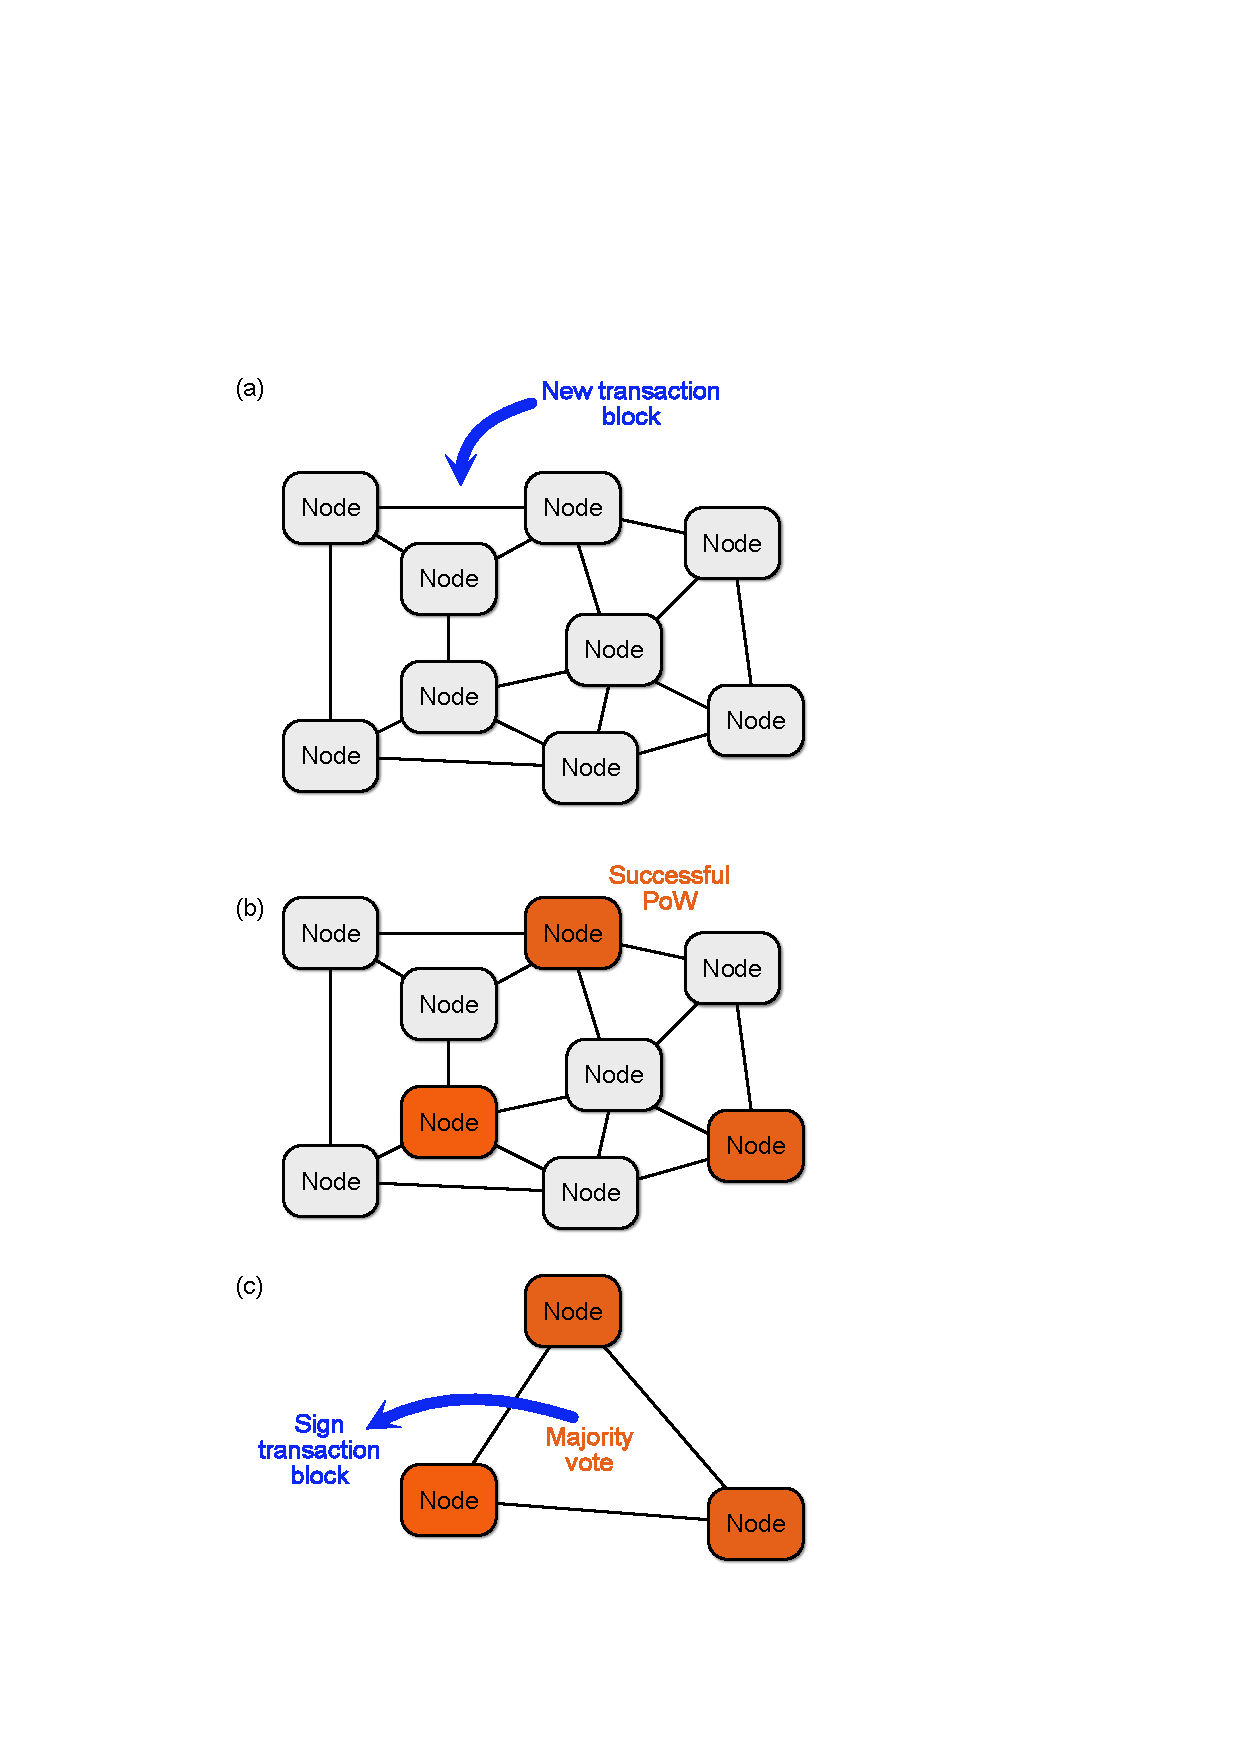
\includegraphics[width=0.8\columnwidth]{figures/distributed_consensus}
\caption{A distributed consensus protocol relying on proof of work to authenticate a blockchain transaction. (a) A network of participating nodes all independently attempt to solve the  proof-of-work problem -- such as the partial pre-image of a hash function -- associated with a new transaction. (b) Due to the unstructured nature of the proof-of-work problem, which nodes successfully solve the problem is inherently randomised, minimising the risk of collusion. (c) The subset of nodes successfully solving the problem sign off on a transaction using digital signatures. The transaction is committed to the blockchain in accordance with a majority vote by consensus participants. Dishonest participants --- ones who vote against the majority --- do not receive their mining reward, thereby incentivising honesty.} \label{fig:distributed_consensus}
\end{figure}

\subsection{Smart contracts}

Many contemporary blockchains accommodate for \emph{smart contracts}, transactions associated with executable code that specify if and under what circumstances the transaction should be executed. This does not rely on any underlying changes to the cryptographic primitives being employed. Rather, it is a higher level abstract layer that sits on top of a protocol relying on existing consensus techniques. Consequently, smart contract platforms are subject to the same vulnerabilities as their underlying blockchain protocol.

\subsection{Distributed autonomous organisations (DAOs)}

One futuristic but currently under-utilised application of smart contract enabled blockchains is the creation of \emph{distributed autonomous organisations} (DAOs). Here we take an entire organisational structure, replacing its administrative components with a framework of smart contracts that algorithmically define and enforce the operational aspects of the organisation. For example, there could be smart contracts associated with payment upon achieving KPIs, or ones enabling members to engage in collective organisational decision making that effectively enforce organisational hierarchy.

DAOs are effectively a further layer of abstraction built on top of a smart contract enabled blockchain. Consequently, their viability and integrity is subject to the same vulnerabilities as the underlying blockchain implementation.